\documentclass[journal,12pt,twocolumn]{IEEEtran}
\usepackage{setspace}
\usepackage{gensymb}
\usepackage{xcolor}
\usepackage{caption}
\singlespacing
\usepackage{siunitx}
\usepackage[cmex10]{amsmath}
\usepackage{mathtools}
\usepackage{hyperref}
\usepackage{amsthm}
\usepackage{mathrsfs}
\usepackage{txfonts}
\usepackage{stfloats}
\usepackage{cite}
\usepackage{cases}
\usepackage{subfig}
\usepackage{longtable}
\usepackage{multirow}
\usepackage{enumitem}
\usepackage{bm}
\usepackage{mathtools}
\usepackage{listings}
\usepackage{tikz}
\usetikzlibrary{shapes,arrows,positioning}
\usepackage{circuitikz}
\renewcommand{\vec}[1]{\boldsymbol{\mathbf{#1}}}
\DeclareMathOperator*{\Res}{Res}
\renewcommand\thesection{\arabic{section}}
\renewcommand\thesubsection{\thesection.\arabic{subsection}}
\renewcommand\thesubsubsection{\thesubsection.\arabic{subsubsection}}

\renewcommand\thesectiondis{\arabic{section}}
\renewcommand\thesubsectiondis{\thesectiondis.\arabic{subsection}}
\renewcommand\thesubsubsectiondis{\thesubsectiondis.\arabic{subsubsection}}
\hyphenation{op-tical net-works semi-conduc-tor}

\lstset{
language=Python,
frame=single, 
breaklines=true,
columns=fullflexible
}
\begin{document}
\theoremstyle{definition}
\newtheorem{theorem}{Theorem}[section]
\newtheorem{problem}{Problem}
\newtheorem{proposition}{Proposition}[section]
\newtheorem{lemma}{Lemma}[section]
\newtheorem{corollary}[theorem]{Corollary}
\newtheorem{example}{Example}[section]
\newtheorem{definition}{Definition}[section]
\newcommand{\BEQA}{\begin{eqnarray}}
\newcommand{\EEQA}{\end{eqnarray}}
\newcommand{\define}{\stackrel{\triangle}{=}}
\newcommand{\myvec}[1]{\ensuremath{\begin{pmatrix}#1\end{pmatrix}}}
\newcommand{\mydet}[1]{\ensuremath{\begin{vmatrix}#1\end{vmatrix}}}
\bibliographystyle{IEEEtran}
\providecommand{\nCr}[2]{\,^{#1}C_{#2}} % nCr
\providecommand{\nPr}[2]{\,^{#1}P_{#2}} % nPr
\providecommand{\mbf}{\mathbf}
\providecommand{\pr}[1]{\ensuremath{\Pr\left(#1\right)}}
\providecommand{\qfunc}[1]{\ensuremath{Q\left(#1\right)}}
\providecommand{\sbrak}[1]{\ensuremath{{}\left[#1\right]}}
\providecommand{\lsbrak}[1]{\ensuremath{{}\left[#1\right.}}
\providecommand{\rsbrak}[1]{\ensuremath{{}\left.#1\right]}}
\providecommand{\brak}[1]{\ensuremath{\left(#1\right)}}
\providecommand{\lbrak}[1]{\ensuremath{\left(#1\right.}}
\providecommand{\rbrak}[1]{\ensuremath{\left.#1\right)}}
\providecommand{\cbrak}[1]{\ensuremath{\left\{#1\right\}}}
\providecommand{\lcbrak}[1]{\ensuremath{\left\{#1\right.}}
\providecommand{\rcbrak}[1]{\ensuremath{\left.#1\right\}}}
\theoremstyle{remark}
\newtheorem{rem}{Remark}
\newcommand{\sgn}{\mathop{\mathrm{sgn}}}
\newcommand{\rect}{\mathop{\mathrm{rect}}}
\newcommand{\sinc}{\mathop{\mathrm{sinc}}}
\providecommand{\abs}[1]{\left\vert#1\right\vert}
\providecommand{\res}[1]{\Res\displaylimits_{#1}} 
\providecommand{\norm}[1]{\lVert#1\rVert}
\providecommand{\mtx}[1]{\mathbf{#1}}
\providecommand{\mean}[1]{E\left[ #1 \right]}
\providecommand{\fourier}{\overset{\mathcal{F}}{ \rightleftharpoons}}
\providecommand{\ztrans}{\overset{\mathcal{Z}}{ \rightleftharpoons}}
\providecommand{\system}[1]{\overset{\mathcal{#1}}{ \longleftrightarrow}}
\newcommand{\solution}{\noindent \textbf{Solution: }}
\providecommand{\dec}[2]{\ensuremath{\overset{#1}{\underset{#2}{\gtrless}}}}
\let\StandardTheFigure\thefigure
\def\putbox#1#2#3{\makebox[0in][l]{\makebox[#1][l]{}\raisebox{\baselineskip}[0in][0in]{\raisebox{#2}[0in][0in]{#3}}}}
     \def\rightbox#1{\makebox[0in][r]{#1}}
     \def\centbox#1{\makebox[0in]{#1}}
     \def\topbox#1{\raisebox{-\baselineskip}[0in][0in]{#1}}
     \def\midbox#1{\raisebox{-0.5\baselineskip}[0in][0in]{#1}}

\vspace{3cm}
\title{Conic Assignment}
\author{Gautam Singh}
\maketitle
\bigskip

\begin{abstract}
    This document contains the solution to Question 6 of Exercise 5 in Chapter
    11 of the class 11 NCERT textbook.
\end{abstract}

\begin{enumerate}
    \item Find the area of the triangle formed by the lines joining the vertex 
    of the parabola 
    \begin{align}
        x^2 = 12y
        \label{eq:parabola}
    \end{align}
    to the ends of its latus rectum.

    \solution Rewriting \eqref{eq:parabola} in matrix form,
    \begin{align}
        \vec{x}^\top\myvec{1&0\\0&0}\vec{x} + 2\myvec{0&-6}\vec{x} = 0
        \label{eq:parabola-mtx}
    \end{align}
    Since the parabola is clearly symmetric about the $y$-axis, we see that
    the directrix is parallel to the $x$-axis, thus
    \begin{align}
        \vec{n} = \myvec{0\\1}
        \label{eq:n}
    \end{align}
    Using the standard definition of the conic and equating $\vec{u}$ and $f$,
    \begin{align}
        \myvec{0\\-6} &= c\myvec{0\\1} - \vec{F} \label{eq:u-eqn} \\
        0 &= \norm{\vec{F}}^2 - c^2 \label{eq:f-eqn}
    \end{align}
    From \eqref{eq:u-eqn}, we have
    \begin{align}
        \vec{F} = \myvec{0\\c+6}
        \label{eq:F-c}
    \end{align}
    Using \eqref{eq:F-c} in \eqref{eq:f-eqn},
    \begin{align}
        \brak{c+6}^2&=c^2 \\
        \implies c&=-3
        \label{eq:c-sol}
    \end{align}
    Thus,
    \begin{align}
        \vec{F} = \myvec{0\\3}
    \end{align}
    The latus rectum of the parabola is the chord passing through the focus 
    parallel to the directrix. Its equation is given by
    \begin{align}
        \myvec{0&1}\vec{x} = \myvec{0&1}\myvec{0\\3} = 3
        \label{eq:latus-rectum}
    \end{align}
    Hence, for $\lambda \in \mathbb{R}$,
    \begin{align}
        \vec{x} = \lambda\myvec{1\\0} + \myvec{0\\3} = \myvec{\lambda\\3}
        \label{eq:x-general}
    \end{align}
    Adding \eqref{eq:parabola-mtx} to 12 times \eqref{eq:latus-rectum}, and
    using \eqref{eq:x-general}
    \begin{align}
        \vec{x}^\top\myvec{1&0\\0&0}\vec{x} &= 36 \\
        \implies \lambda^2 &= 36 \\
        \implies \lambda &= \pm 6
        \label{eq:x-latus}
    \end{align}
    Thus, the ends of the latus rectum are
    \begin{align}
        \vec{x} = \myvec{\pm 6\\3}
    \end{align}
    Since the vertex of the parabola is at $\vec{P} = \myvec{0\\0}$,
    we see that the area of the required triangle is
    \begin{align}
        A = \frac{1}{2}\mydet{6&3\\-6&3} = 18\ \textrm{sq. units}
    \end{align}
    The situation is illustrated in Fig. \ref{fig:parabola}, plotted using the
    Python code \texttt{codes/parabola.py}.
    \begin{figure}[!ht]
        \centering
        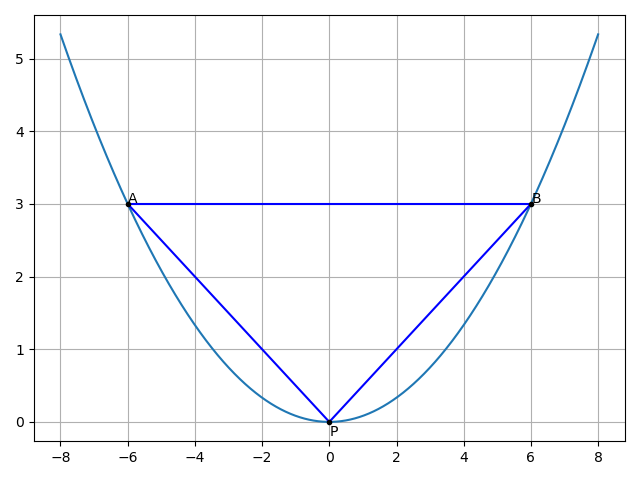
\includegraphics[width=\columnwidth]{figs/parabola.png}
        \caption{$PAB$ is the triangle whose area is to be found.}
        \label{fig:parabola}
    \end{figure}
\end{enumerate}
\end{document}
